\documentclass[aspectratio=1610]{beamer}
\mode<presentation>
\usetheme{Madrid}
\usecolortheme{seahorse}
% \usepackage[table]{xcolor}
\usepackage{multimedia}
\usepackage{media9}
\usepackage[utf8]{inputenc}
\usepackage{amsmath}
\usepackage{lmodern}
% \usepackage[usenames, dvipsnames]{color}

\usepackage{arydshln}
\usepackage{url}
\usepackage[absolute,overlay]{textpos}
\usepackage[texcoord,grid,gridunit=cm,gridcolor=red!50,subgridcolor=green!50]{eso-pic}
\setlength{\TPHorizModule}{\textwidth}
\setlength{\TPVertModule}{\textwidth}

\graphicspath{{plots/}}

\setbeamercolor{CBwonb}{fg=white,bg=white!10!blue}
\setbeamercolor{CBronb}{fg=red,bg=white!10!blue}

\usepackage{tikz}
\usetikzlibrary{shapes,arrows,positioning}
\tikzstyle{startstop} = [rectangle, rounded corners, minimum width=1cm, minimum height=0.1cm,text centered, text width=2.5cm, draw=black, fill=red!30]
\tikzstyle{io} = [trapezium, trapezium left angle=70, trapezium right angle=110, minimum width=1cm, minimum height=0.1cm, text centered, text width=2.5cm, draw=black, fill=blue!30]
\tikzstyle{process} = [rectangle, minimum width=1cm, minimum height=0.1cm, text centered,text width=2.5cm, draw=black, fill=orange!30]
\tikzstyle{decision} = [circle, minimum width=1cm, minimum height=0.1cm, text centered,text width=2.5cm, draw=black, fill=green!30]
\tikzstyle{arrow} = [thick,->,text centered, color=blue, text width=2cm,>=stealth]

\newcommand{\Msun}{~{\rm M_\sun}}
\newcommand{\hMsun}{~h^{-1}\>{\rm M_\odot}}
\newcommand{\Mpc}{~h^{-1}~{\rm Mpc}}
\newcommand{\Kpc}{~h^{-1}~{\rm kpc}}


\title[]{The Large Scale Environments}
\subtitle{The large-scale distribution of baryons inside the cosmological
hydrodynamical simualtions.}
\author[Email: weiguang.cui@uam.es]{{\Large \bf Weiguang Cui},\inst{*} \footnote{\url{https://weiguangcui.github.io}}}
\institute[]{
  \inst{*}
  Departamento de F\'isica Te\'{o}rica, \\
  Universidad Aut\'{o}noma de Madrid, 28049 Madrid, Spain
}
\date[]{The HUBS workshop, Shanghai. \\  October, 16, 2018}
\logo{
\includegraphics[height=1cm]{logo_uam.jpg}}

%%%%%%%%%%%%%%%%%%%%%%%%%%%%%%%%%%%%%%%%%%%%%%%%%%%%%%%%%%%%%%%%%%%%%%%%%
\begin{document}
  \frame{\titlepage}

%----------------------------------
\section{Introduction} \label{sec:1}

\begin{frame}
  \frametitle{Background: the distribution of galaxies at large-scale}
  \framezoom<1><2>(2.5cm,3cm)(2.5cm,2.5cm)
  \begin{figure}
    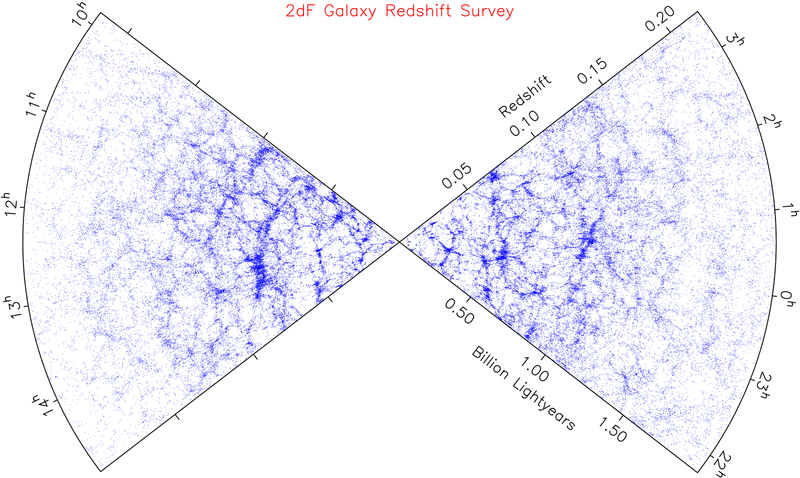
\includegraphics[width=0.8\textwidth]{2dFzcone.jpg}
  \end{figure}

  Credit: Yang et al. 2005
\end{frame}

\begin{frame}
  \frametitle{Background: the distribution of dark matter at large-scale}
  \framezoom<1><2>[](5cm,3.5cm)(1.5cm,1.5cm)
  \begin{figure}
    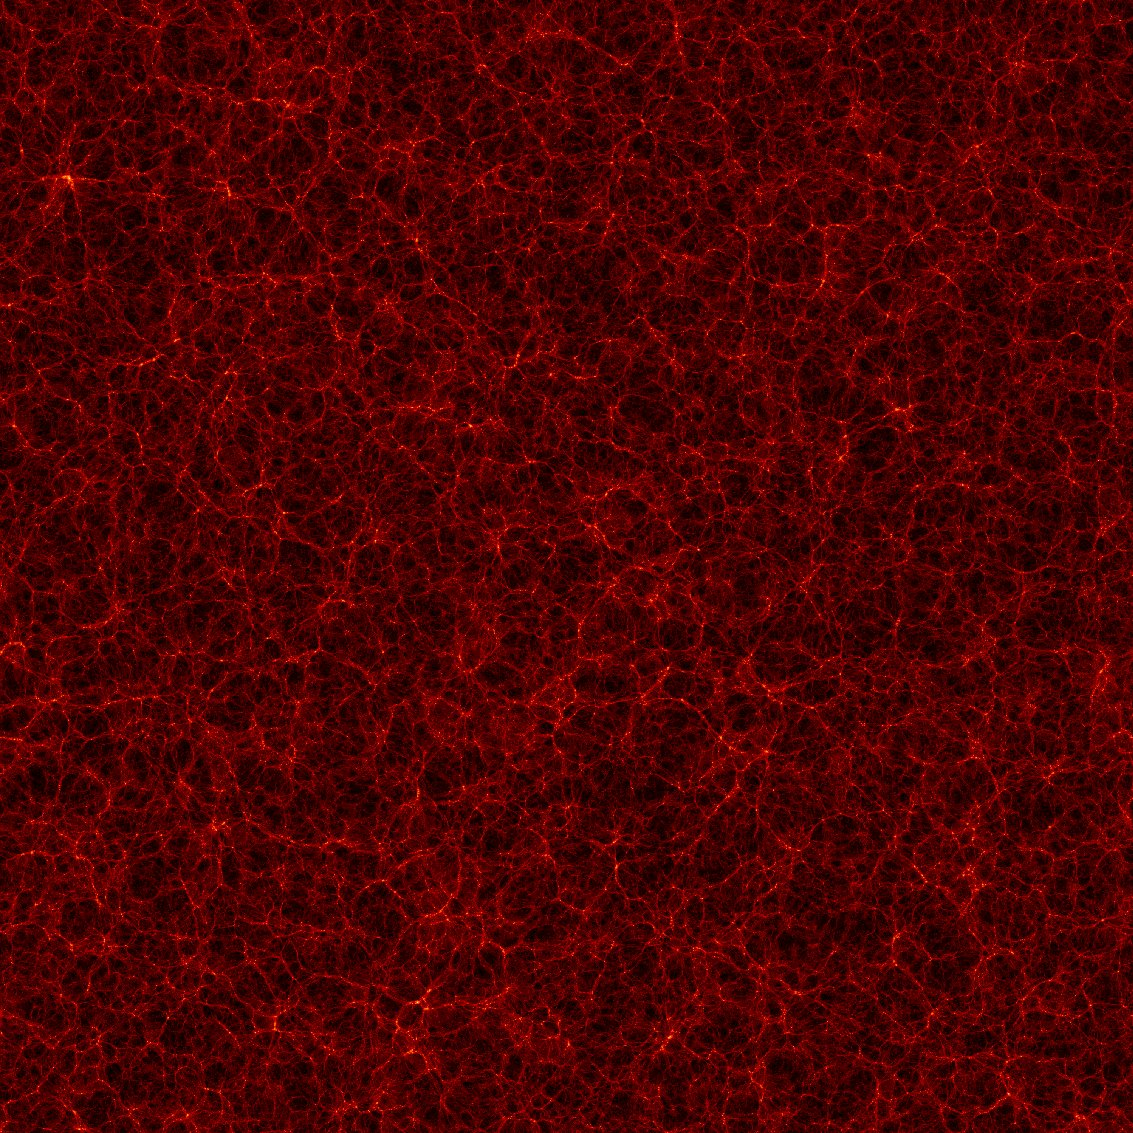
\includegraphics[width=0.55\textwidth]{mdpl.jpg}
  \end{figure}
  Credit: MultiDark Planck simulation
\end{frame}

\begin{frame}
  \frametitle{Background: the fractions}
  \begin{figure}
    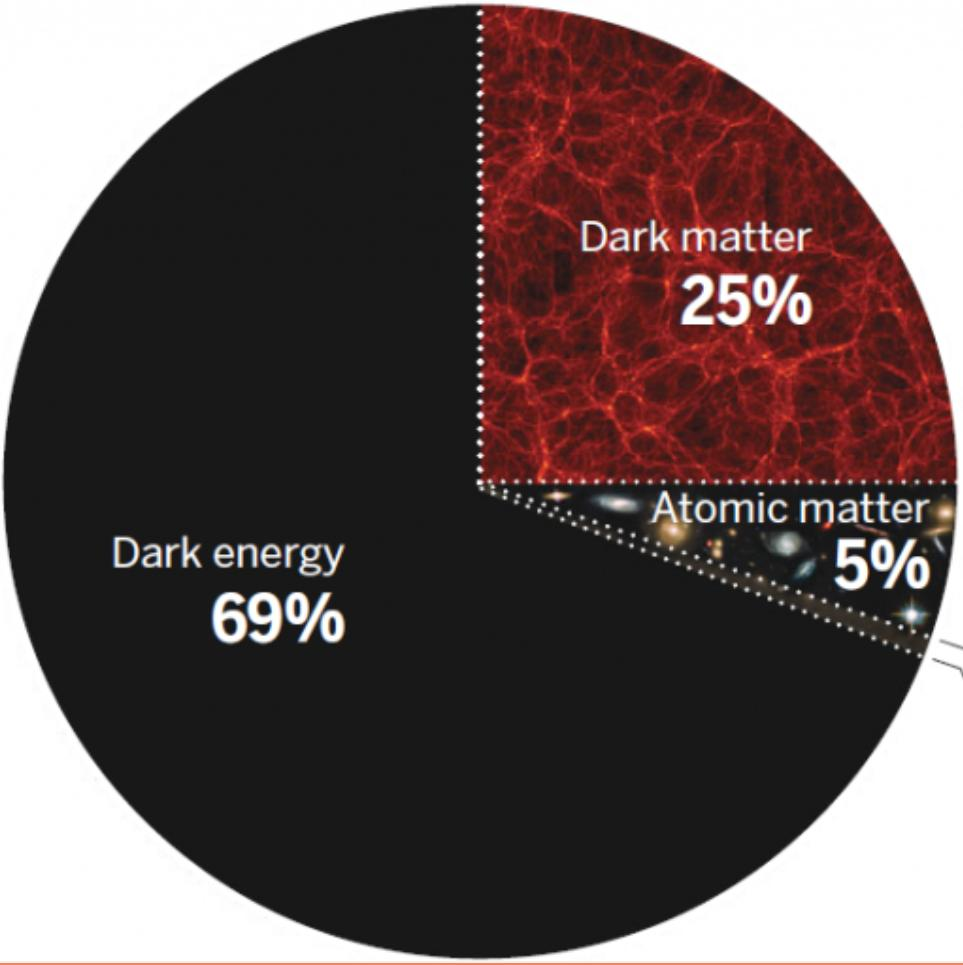
\includegraphics[width=0.55\textwidth]{fraction.jpg}
  \end{figure}
  \begin{textblock*}{4cm}(12.3cm,6cm)
    {\color{red}{Stars only account for $\sim$0.07\%}}
  \end{textblock*}
\end{frame}
\begin{frame}{Background: where is the others??}
  \begin{figure}
    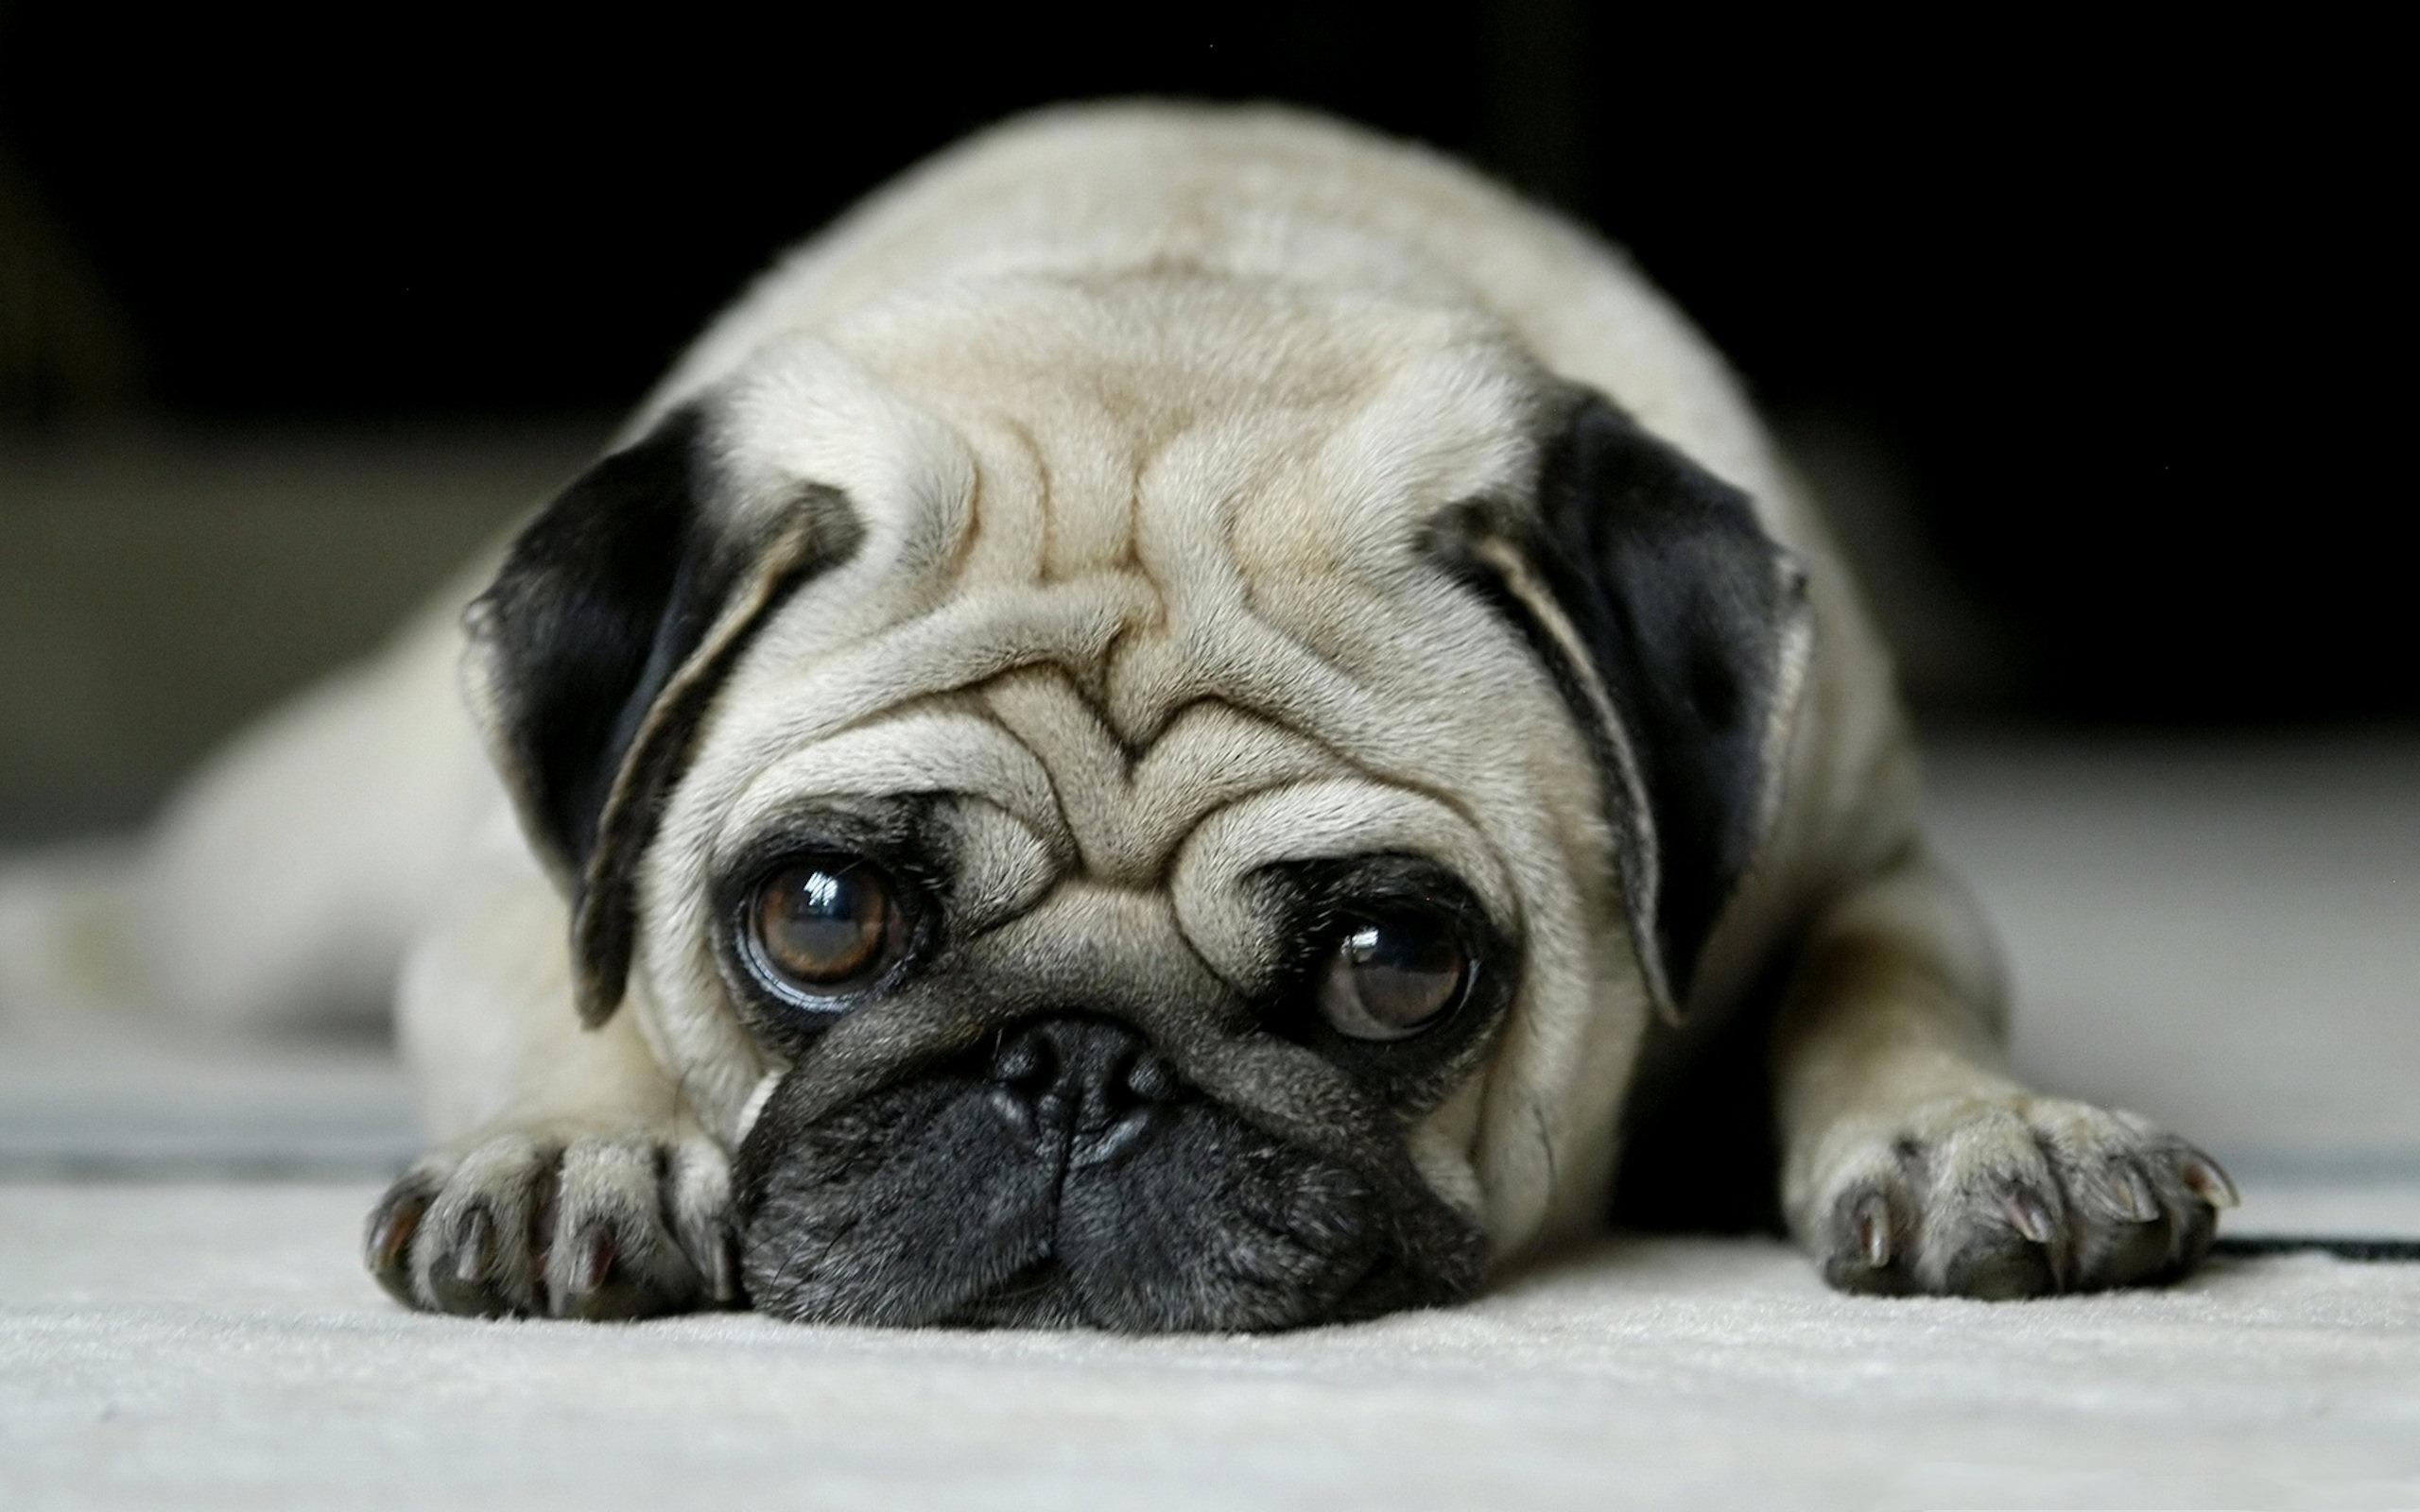
\includegraphics[width=0.8\textwidth]{lonely-dog.jpg}
  \end{figure}
  \only<2>{
    \begin{textblock*}{15cm}(4cm,3cm)
      {\Huge \color{red}{WHIM: WHy I'M here?}}
    \end{textblock*}
  }
\end{frame}

\begin{frame}
  \frametitle{What is in this talk?}
  \begin{itemize}
    \item<1-> How to classify the large-scale environment?
    \item<2-> The theoretical models for this study.
    \item<3-> What does the model say about the baryon distribution?
    \item<4-> Conclusion and future prospects.
  \end{itemize}
  % \only<1>{
  %   \begin{center}
  %     {\Large \bf The {\sc nIFTy} galaxy cluster comparison project}\footnote{\scriptsize Ref: Sembolini et al. 2016a,b; Elahi et al. 2016; Cui et al. 2016; Arthur et al. 2017}
  %   \end{center}
  %   \alert{11} different (in both algorithms and baryon models) simulation codes are used to simulate the same galaxy cluster.
  % }
  % \only<2>{
  %   \begin{center}
  %     {\Large \bf What did we find? I}
  %   \end{center}
  %   {\scriptsize
  %   \begin{itemize}
  %     \item The modern SPH codes produce correct entropy profiles as AMR, moving mesh.
  %     \item The baryon models have larger effects than the fluid simulating techniques by mixing the entropy profiles.
  %   \end{itemize}}
    % \begin{figure}
    %   \vspace{-0.2cm}
    %   \includegraphics<2>[width=0.36\textwidth]{nifty-entropy.png}
    %   \includegraphics<2>[width=0.45\textwidth]{nifty-entropy-fp.png}\vspace{-0.4cm}
    %   % \caption{{\scriptsize Entropy profile. Ref: Sembolini et al. 2016a,b}}
    % \end{figure}
    % \begin{textblock}{0.12}(0.01,0.3)
    %   {\scriptsize  Entropy profile. \\ Ref: Sembolini et al. 2016a,b.}
    % \end{textblock}
  % }
\end{frame}

\section{The classification methods}
\begin{frame}
  \frametitle{The classification method -- Vweb}

  \begin{itemize}
    \item The most massive ($M_{vir} > 8\times 10^{14} \hMsun$) 324 clusters are selected from the MultiDark simulation(MDPL2)\footnote{\url{https://www.cosmosim.org}}.
    \item 324 zoomed-in ICs are generated by cutting a spherical region with a radius of \alert{$15 \Mpc$} from the cluster center.
    \item[]
      \begin{table}
        \fontsize{10}{10}\selectfont
        \caption{Parameters of the Three Hundred simulations}
        \begin{tabular}{lll}
          \hline
          Parameter& Value & Description\\
          \hline
          $\Omega_M$ & 0.307 & Total Matter density parameter\\
          $\Omega_B$ & 0.048 & Baryon density parameter\\
          $\Omega_\Lambda$ & 0.693 & Cosmological Constant density parameter\\
          $h$ & 0.678  & Hubble constant in units of 100 km/s/Mpc\\
          $\sigma_8$ & 0.823 & Normalization of Power spectrum\\
          $n_s$ & 0.96  & Power index\\
          % $f_B$ & 0.0696&  Cosmic Baryon Fraction\\
          $z_{init}$ & 120 & Initial redshift of the simulations \\
          $\epsilon_{phys}$ & 6.5 & Plummer equivalent softening in $\Kpc$ \\
          % Box size & 1 $h^{-1} Gpc$ (15 $\Mpc$) & The MDPL2 simulation box on one side (the radius for each re-simulation region) \\
          Particle mass & $2.36 \ (12.7) $ & gas (dark matter) particle mass in [$10^8 \hMsun$]\\
          \hline
        \end{tabular}
      \end{table}
\end{itemize}
% \vspace{-0.6cm}
\end{frame}

\begin{frame}
  \frametitle{The classification method -- Pweb}
  \begin{columns}[t]
    \begin{column}{0.55\textwidth}
      \begin{block}{hydrodynamical simulations with baryonic models:}
        {\sc Gadget-\alert{MUSIC}}: classic SPH method. Radiative cooling, star formation with both thermal and kinetic Supernove (SN) feedback.

        {\sc Gadget-\alert{X}}: modern SPH with the Wendland C4 kernel. Gas cooling with metal contributions, star formation with chemical enrichment, SN feedback with AGB phase, and AGN feedback.

        {\sc GIZMO:} running.

        {\sc Gadget-PESPH:} running.
      \end{block}
    \end{column}
    \begin{column}{0.4\textwidth}
      \begin{block}{SAMs from MultiDark-Galaxies:}
        See Alexander's talk for more details of {\sc Galacticus}, {\sc SAG} (see also sofia's talk) and {\sc SAGE} (see also Darren's talk).

        Notes: We select these catalogues from the same regions as the hydrodynamical simulations.
      \end{block}
    \end{column}
  \end{columns}
  % A coupling with MultiDark-Galaxies
\end{frame}

\section{simulations}
\begin{frame}{The cosmological hydrodynamical simulations}

\end{frame}

\section{Results}
\begin{frame}{An illustriation}
  \begin{figure}
    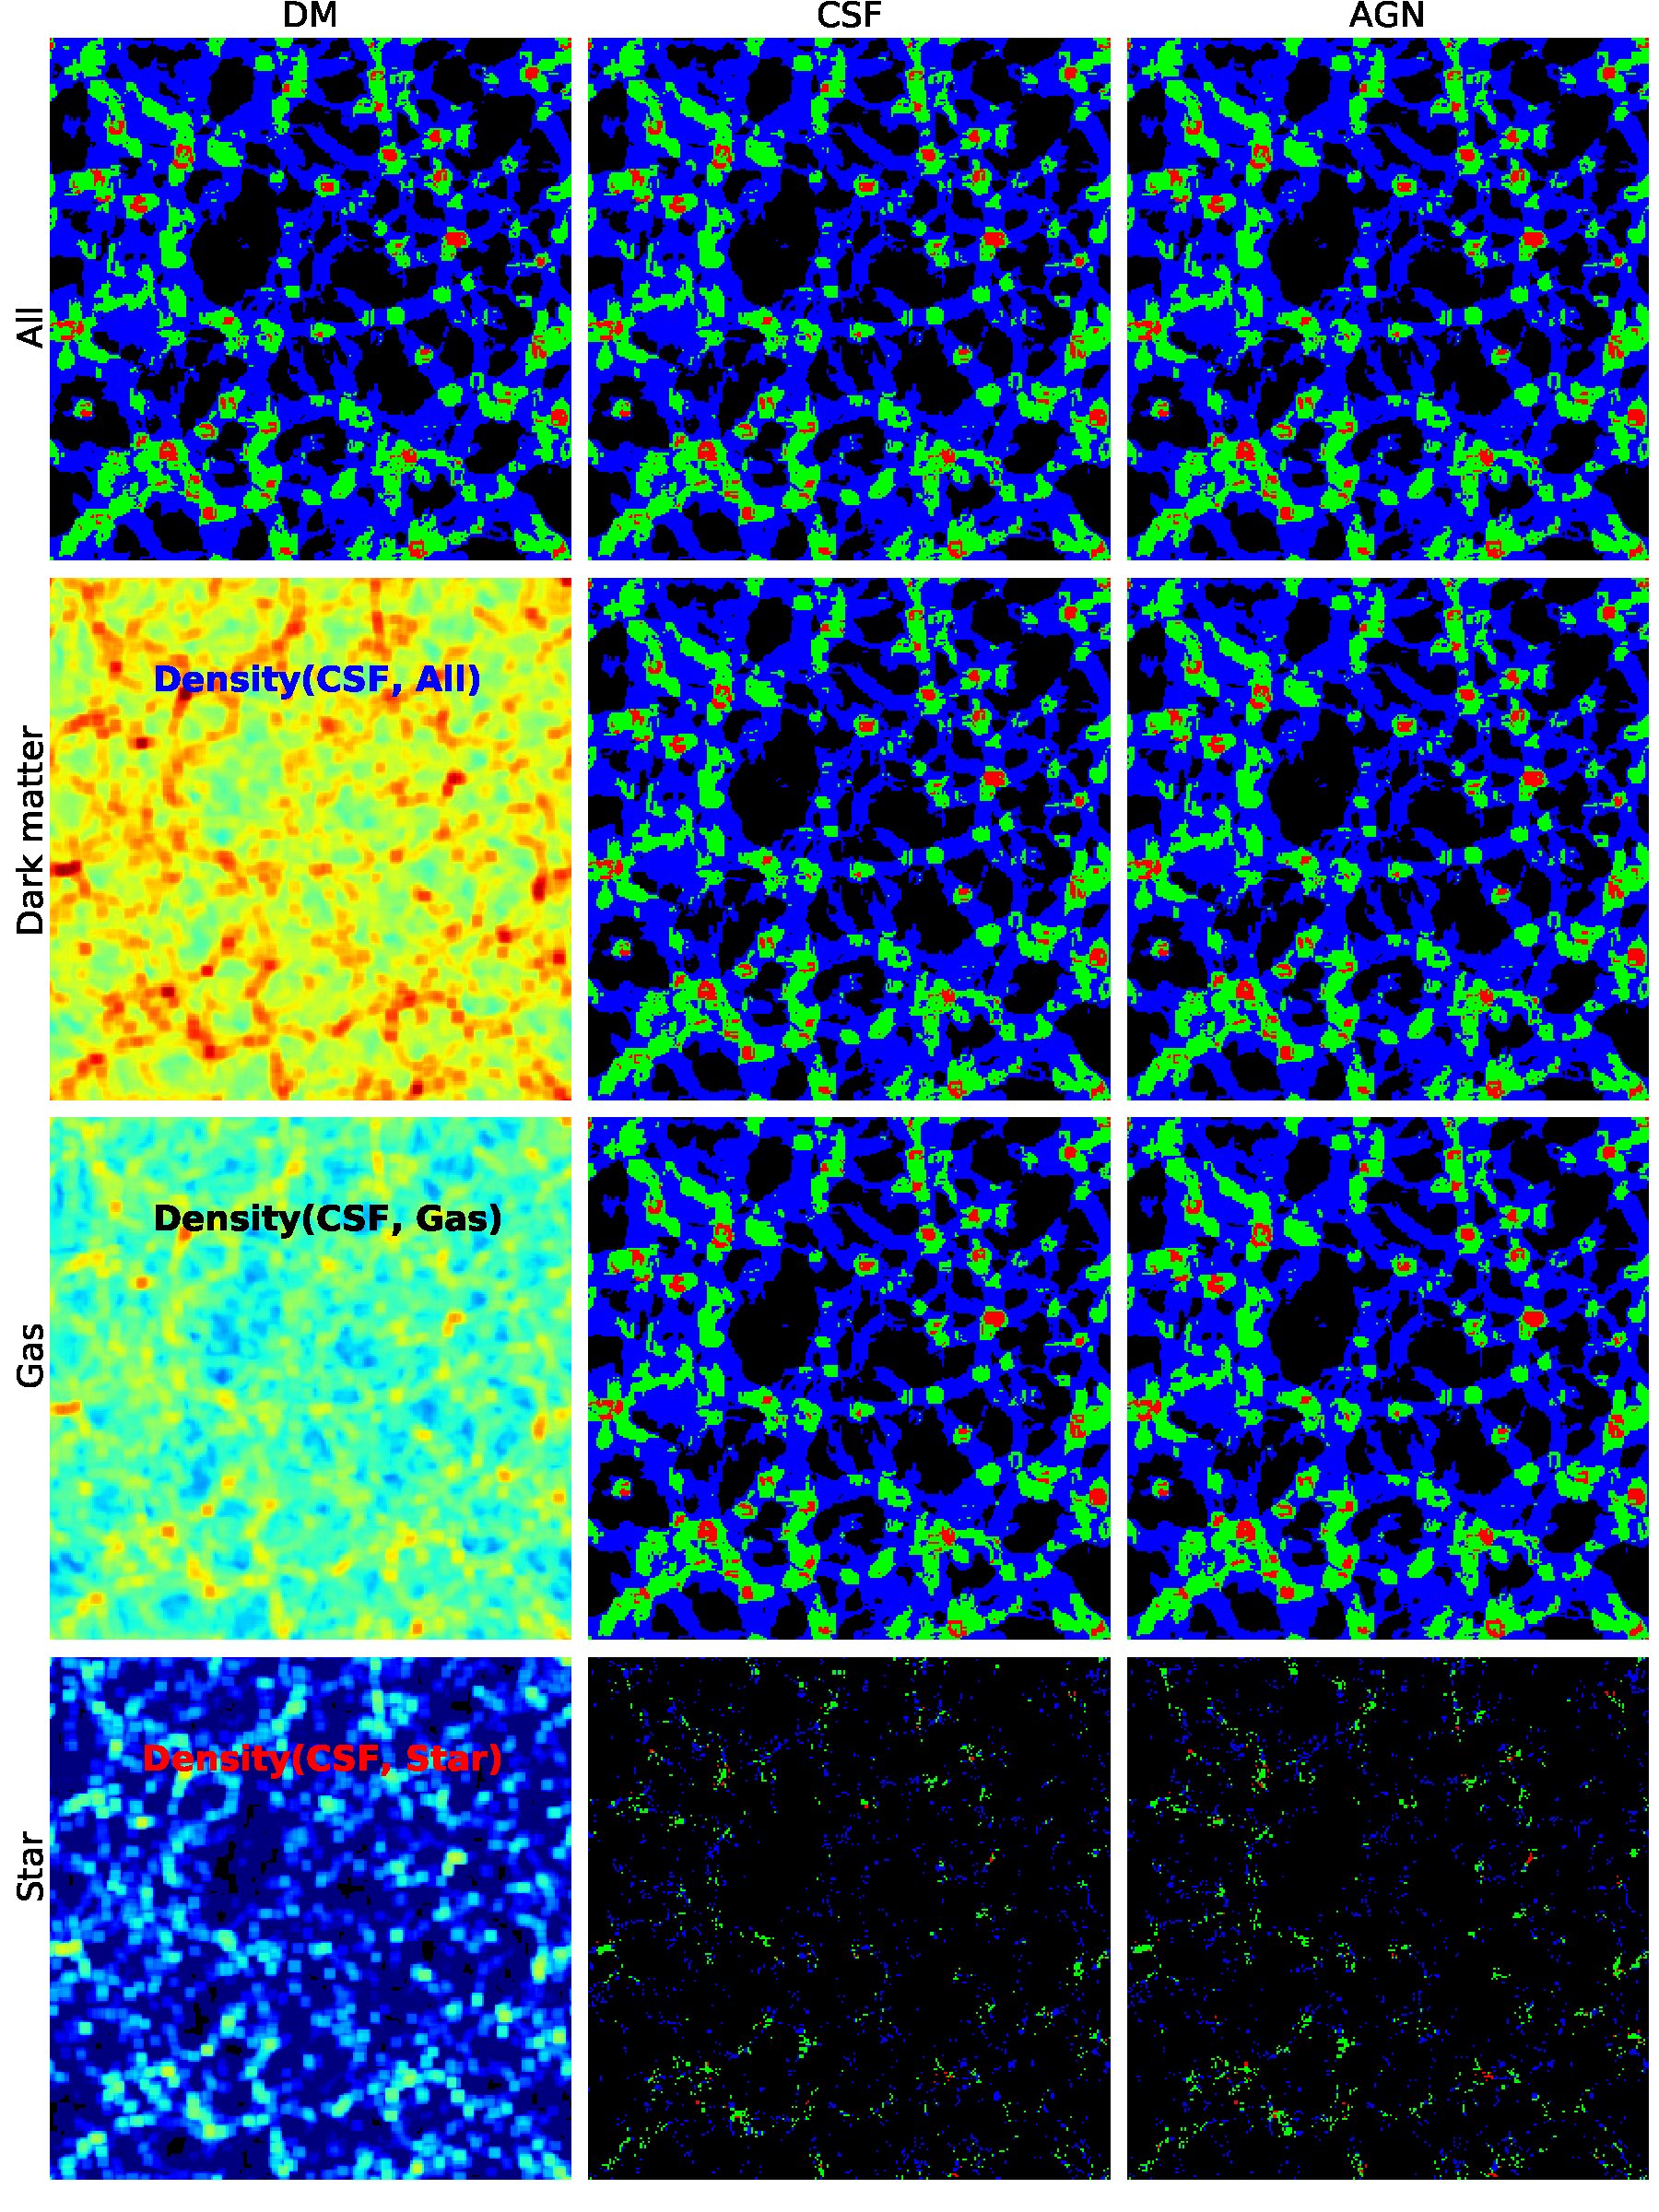
\includegraphics[width=0.33\linewidth]{image_show_V}
  \end{figure}
  \begin{textblock*}{4cm}(12.3cm,6cm)
    {Cui et al. 2018, Paper I, z=0}
  \end{textblock*}
\end{frame}

\begin{frame}{The fractions}
  \begin{figure}
    \includegraphics<1>[width=\linewidth]{Fractions-BE}
    \includegraphics<2>[width=\linewidth]{Fractions-gasweb}
    \caption{The mass and volume fractions of these large-scale environments}
  \end{figure}
  \begin{textblock*}{4cm}(12.3cm,6cm)
    {Cui et al. 2018, Paper I, z=0}
  \end{textblock*}
\end{frame}

\begin{frame}
  \begin{textblock*}{8cm}(6.3cm,6cm)
    {\Huge Primarily results from Paper II}
  \end{textblock*}
\end{frame}

\begin{frame}{An illustriation: redshift evolution}
  \begin{figure}
    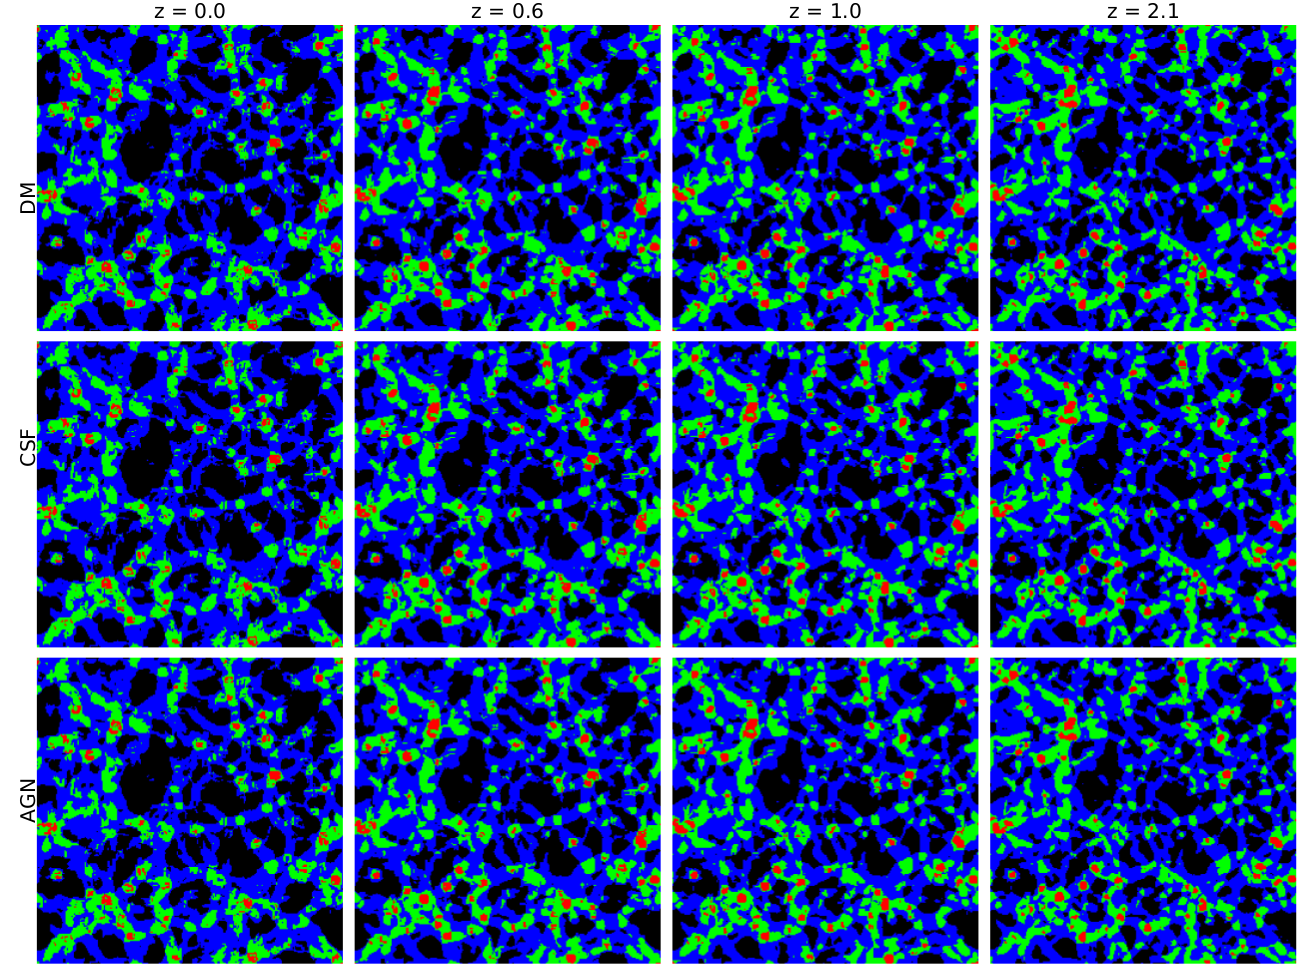
\includegraphics[width=0.6\linewidth]{Evolution-illustriation}
  \end{figure}
\end{frame}



\section{conclusion and future prospections}
\begin{frame}
  \frametitle{Conclusion}
  {\Large
  \begin{itemize}
    \item The baryons have a negligible impact on the halo mass for both $M_{200}$ and $M_{500}$.
    \item $\sim 20 \%$ of the complete sample is relaxed clusters, 26\% (9\%) of the sample is CC for GadgetX (MUSIC).
    \item The baryon fractions are in agreement with the observations at massive halo masses for GadgetX.
    \item The optical relations are in agreement with the observations but the galaxies from more models seem to be a little blue.
    \item The gas relations are in agreement with observations.
  \end{itemize}}
\end{frame}

\begin{frame}
  \frametitle{Future prospects}
  The detailed fractions that we can measure -- connecting hydrodynamical simulations with observations through mock images.
  \begin{itemize}
    \item Optical: pymgal
    \item Xray: pymxc  (More details)
    \item SZ: pymsz
    \item Radio: pymr
  \end{itemize}

  \only<2>{
  Suggestions to HUBS:
  \begin{itemize}
    \item[1] theoretical investigation with pymxc.
    \item[2] Application to cosmology.
  \end{itemize}}
\end{frame}
\end{document}
